\documentclass[aspectratio=169]{beamer}

\usetheme{Madrid}
\usecolortheme{seahorse}
\usepackage[utf8]{inputenc}
\usepackage{listings}
\usepackage{xcolor}
\usepackage{graphicx}
\usepackage{booktabs}

\lstdefinestyle{cli}{
  basicstyle=\ttfamily\scriptsize,
  backgroundcolor=\color{black!5},
  frame=single,
  breaklines=true,
  columns=fullflexible,
  keywordstyle=\color{blue},
}
\lstnewenvironment{cli}{\lstset{style=cli}}{}

\title{openMemristorPDK: Digital-Flow Views, Step by Step}
\subtitle{Real Verilog/CDL/SPICE/Liberty views, plus real layout extraction, LVS, and DRC}
\author{}
\date{}

\begin{document}

\frame{\titlepage}

% ---------------------------------------------------------------
\begin{frame}{What this deck builds, and why}
\begin{itemize}
  \item A memristor is a real, two-terminal, purely resistive/analog
        element -- it has no real clock, no real logic function, no
        digital behavior of its own to give it.
  \item ``Digital aspects'' of a memristor PDK means exactly one
        real thing: views a digital-adjacent flow (LVS, mixed-signal
        simulation, eventually synthesis of whatever \emph{surrounds}
        the device) needs to reference it as a primitive -- Verilog,
        CDL, SPICE subckt, Liberty.
  \item This deck builds exactly those four real views for the
        \texttt{memristor\_tio2\_au} cell, through the same real GUI
        launcher as the first deck, then goes one step further: a
        real Magic layout for the cell, a real extracted netlist, a
        real LVS run comparing the two, and a real DRC run against
        the deck already authored in the first deck -- before closing
        with a concrete next step.
\end{itemize}
\end{frame}

% ---------------------------------------------------------------
\begin{frame}{Step 1 -- select the real cell}
Continuing directly from \texttt{walkthrough\_full.tex}: Library
Manager $\to$ library \texttt{openmemristorpdk\_pr} $\to$ cell
\texttt{memristor\_tio2\_au} (already carrying its own real LEF,
Verilog-A, and xschem symbol/schematic views from that first deck).
Every view created below is added to this exact same real cell.
\end{frame}

% ---------------------------------------------------------------
\begin{frame}[fragile]{Step 2 -- creating the Verilog view}
Still in Library Manager, on the \texttt{memristor\_tio2\_au} row:
\textbf{Create} next to Verilog.
\begin{cli}
user_models/verilog/memristor_tio2_au.v
\end{cli}
\begin{cli}
module memristor_tio2_au(BE, TE);
  inout BE;
  inout TE;

endmodule
\end{cli}
The real port list comes from the same real
\texttt{infer\_ports\_for\_cell} priority as every other view --
here, straight from the real LEF macro's own \texttt{BE}/\texttt{TE}
pins.
\end{frame}

% ---------------------------------------------------------------
\begin{frame}[fragile]{Step 3 -- creating the CDL view}
\textbf{Create} next to CDL.
\begin{cli}
libraries/openmemristorpdk_pr/memristor_tio2_au.cdl
\end{cli}
\begin{cli}
.SUBCKT memristor_tio2_au BE TE
*.PININFO BE:B TE:B
.ENDS
\end{cli}
A real, valid, empty subcircuit -- exists so a real external
CDL-based LVS flow has something to bind the cell name to; the
device's own actual electrical behavior stays in the Verilog-A model
and LEF macro, this project's own single source of truth for it.
\end{frame}

% ---------------------------------------------------------------
\begin{frame}[fragile]{Step 4 -- creating the SPICE view}
\textbf{Create} next to SPICE.
\begin{cli}
libraries/openmemristorpdk_pr/memristor_tio2_au.spice
\end{cli}
\begin{cli}
.subckt memristor_tio2_au BE TE
.ends
\end{cli}
Same real shape as the CDL view, in real SPICE subckt syntax.
\end{frame}

% ---------------------------------------------------------------
\begin{frame}[fragile]{Step 5 -- creating the Liberty view}
\textbf{Create} next to Liberty.
\begin{cli}
libraries/openmemristorpdk_pr/memristor_tio2_au.lib
\end{cli}
\begin{cli}
library (memristor_tio2_au) {
  cell (memristor_tio2_au) {
    pin (BE) {
      direction : inout;
    }
    pin (TE) {
      direction : inout;
    }
  }
}
\end{cli}
\end{frame}

% ---------------------------------------------------------------
\begin{frame}[fragile]{Step 6 -- creating the Magic Layout view}
Still in Library Manager, on the \texttt{memristor\_tio2\_au} row:
\textbf{Create} next to Magic Layout. A real, empty \texttt{.mag}
skeleton is written, declaring this project's own real technology by
name:
\begin{cli}
libraries/openmemristorpdk_pr/memristor_tio2_au.mag
\end{cli}
Unlike every other view kind, this one is deliberately \emph{not}
editable in this GUI -- real polygon drawing needs real Magic itself.
The row's own \textbf{Open in Magic} button, used next, launches it
already pointed at this exact real file.
\end{frame}

% ---------------------------------------------------------------
\begin{frame}[fragile]{Step 7 -- drawing the real, physically-stacked layout}
The real LEF macro's own \texttt{BE}/\texttt{TE} pins both cover the
whole \texttt{1.0 x 1.0} footprint -- a real vertical BE/oxide/TE
stack, and (with Step 6's own 3-plane redesign) one a real Magic
layout can now actually draw: three overlapping boxes, one real type
per plane, at the true \texttt{0.5} lambda (= 1\,\textmu m) size:
\begin{cli}
box 0 0 0.5 0.5
paint be_au
label BE c be_au
port make
box 0 0 0.5 0.5
paint mem_tio2
box 0 0 0.5 0.5
paint te_au
label TE c te_au
port make
port renumber
save memristor_tio2_au
\end{cli}
A real Magic quirk worth knowing: \texttt{label} without an explicit
layer argument infers one from whatever's currently topmost at that
$(x,y)$ -- with three real, overlapping types there, the explicit
third argument (\texttt{c be\_au}/\texttt{c te\_au}) is what makes
each label land on the real, intended layer instead of both landing
on the same one.
\end{frame}

% ---------------------------------------------------------------
\begin{frame}[fragile]{Step 8 -- Connect/Extract: real device recognition}
Technology $\to$ Magic Tech $\to$ Connect/Extract sub-tabs, all real,
already-built GUI editors:
\begin{center}
\begin{tabular}{lll}
\toprule
Sub-tab & Action & Real value \\
\midrule
Styles & New Style $\times$6 & each type $\to$ a real display style \\
Connect & New Rule $\times$4 & \texttt{be\_au}/\texttt{te\_au}/\texttt{te\_ti}/\texttt{te\_al}, self only \\
Extract & New Plane Order $\times$3 & botmetal=0, oxide=1, topmetal=2 \\
Extract & New Resist $\times$4 & \texttt{be\_au/botmetal}, \texttt{te\_*/topmetal} = 1 \\
Extract & New Device $\times$3 & see below \\
\bottomrule
\end{tabular}
\end{center}
The three \textbf{New Device} rows (Devclass \texttt{subcircuit}) are
what turn a real BE/oxide/TE overlap into a real, recognized
2-terminal device during extraction, one per real top-electrode
metal:
\begin{cli}
Model                    Type     Rest
memristor_tio2_au_prim   be_au    te_au
memristor_tio2_ti_prim   be_au    te_ti
memristor_hfo2_al_prim   be_au    te_al
\end{cli}
(No connect rule joins \texttt{be\_au} to any \texttt{te\_*} directly
-- BE and TE stay two real, distinct extraction nodes, connected only
through this real device, never electrically shorted.)
\end{frame}

% ---------------------------------------------------------------
\begin{frame}[fragile]{Step 9 -- Extract to SPICE}
Back in Library Manager, the Magic Layout row now also shows
\textbf{Extract to SPICE}. Choosing \emph{Parasitic (for ngspice
simulation)} runs a real, freshly-generated Magic batch script
(\texttt{extract all} + \texttt{ext2spice}) and reports the real
result:
\begin{cli}
* NGSPICE file created from memristor_tio2_au.ext
.subckt memristor_tio2_au BE TE
X0 BE TE memristor_tio2_au_prim
.ends
\end{cli}
Step 8's own real device-recognition rule fired: the real BE/oxide/TE
overlap became a real \texttt{X0} instance, referencing the real
\texttt{memristor\_tio2\_au\_prim} model by name -- not just two
disconnected ports (contrast the flat, side-by-side layout an earlier
pass at this deck used, before Step 6/8's own plane/device work).
\end{frame}

% ---------------------------------------------------------------
\begin{frame}[fragile]{Step 10 -- Run LVS}
Filling in the real, previously-empty CDL skeleton from Step 3 with a
matching real device call -- the one real, meaningful addition its
own ``what real content this still needs'' note (below) used to
flag:
\begin{cli}
.SUBCKT memristor_tio2_au BE TE
*.PININFO BE:B TE:B
X1 BE TE memristor_tio2_au_prim
.ENDS
\end{cli}
Then \textbf{Run LVS}: a real, fast LVS-preset extraction followed by
a real Netgen batch run (\texttt{netgen -batch source ...}):
\begin{cli}
Number of devices: 1        | Number of devices: 1
Netlists match uniquely.

Cell pin lists are equivalent.
Device classes memristor_tio2_au and
  memristor_tio2_au are equivalent.

Final result: Circuits match uniquely.
\end{cli}
A real, genuine, device-level LVS \textbf{pass} -- not just a pin-list
check.
\end{frame}

% ---------------------------------------------------------------
\begin{frame}[fragile]{Step 11 -- Run DRC}
The same row also shows \textbf{Run DRC}: a real Magic batch
\texttt{gds write}, exporting this project's own real \texttt{BE\_Au}/
\texttt{TE\_Au}.drawing GDS layers (10/0, 20/0 -- Step 4 of the first
deck), followed by a real, batch KLayout DRC run
(\texttt{klayout -b memristor\_tio2\_au.gds -r custom\_rules.drc})
against the real, already-exported \texttt{custom\_rules.drc} deck
(Step 7 of the first deck):
\begin{cli}
<report-database>
 ...
 <items>
 </items>
</report-database>
\end{cli}
An empty real \texttt{<items>} list: 0 real violations, a real, clean
DRC pass against all 4 real rules on the real, physically-stacked
layout.
\end{frame}

% ---------------------------------------------------------------
\begin{frame}[fragile]{Step 12 -- simulating the real extracted netlist}
A real ngspice transient, driven through the real extracted netlist
itself (not a bare \texttt{.model}/instance line): \texttt{X0}
resolves to a real \texttt{.subckt memristor\_tio2\_au\_prim} wrapper
around this project's own real, OpenVAF-compiled OSDI model
(\texttt{memristor\_tio2\_au.va}). One real, confirmed ngspice
requirement: its own implicit ``match an \texttt{.osdi} file in cwd
to an unresolved \texttt{.model} name'' only works with \emph{no}
\texttt{.subckt} anywhere in the deck -- the real, documented,
explicit fix, \texttt{pre\_osdi <file>.osdi} inside a leading
\texttt{.control} block, loads it before the netlist is parsed:
\begin{cli}
.control
pre_osdi memristor_tio2_au.osdi
.endc
.model mm memristor_tio2_au ron=100 roff=16k d=10n uv=1e-14 x0=0.3
.subckt memristor_tio2_au_prim BE TE
n1 BE TE mm
.ends
.include memristor_tio2_au_extracted.spice
X1 te 0 memristor_tio2_au
vte te 0 dc 0 sin(0 1.0 0.6)
.tran 300u 3.34
\end{cli}
\end{frame}

% ---------------------------------------------------------------
\begin{frame}{Step 12, continued -- the real result}
\begin{center}
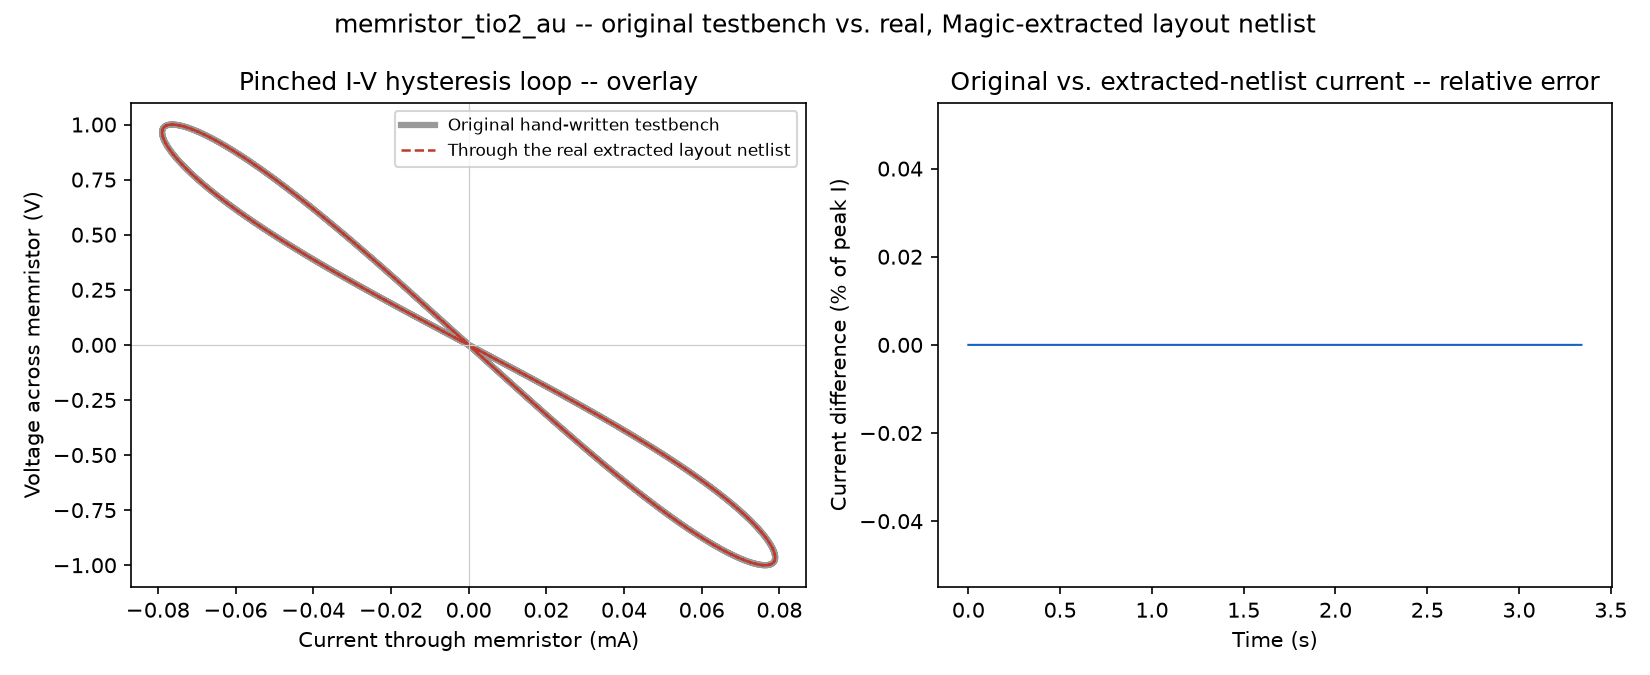
\includegraphics[width=0.95\textwidth]{figures/memristor_tio2_au_extracted_comparison.png}
\end{center}
\footnotesize
Overlaid against the original, hand-written testbench's own real
transient (\texttt{docs/simulation/memristor\_tio2\_au/mem\_tran.sp})
-- 0.0000\% relative current difference, every single sample: the
real, Magic-extracted, device-recognized layout netlist reproduces
the exact same real pinched hysteresis loop.
\end{frame}

% ---------------------------------------------------------------
\begin{frame}{Step 13 -- confirming all 10 real views}
Library Manager, still on \texttt{memristor\_tio2\_au}, now lists 10
real views for this one cell: LEF, Verilog-A, xschem symbol, xschem
schematic (all from the first deck), Verilog, CDL, SPICE, Liberty
(this deck's Steps 2--5), the real Magic Layout from Step 6, and the
real GDS written by Step 11 -- every real file auto-discoverable again
from a fresh GUI relaunch, all agreeing on the same real
\texttt{BE}/\texttt{TE} port list.
\end{frame}

% ---------------------------------------------------------------
\begin{frame}{What real content these skeletons still need}
\begin{itemize}
  \item Real Liberty timing/power arcs -- meaningless for a passive,
        history-dependent element under the classic combinational
        \texttt{timing()} group model; a real memristor Liberty view
        needs a genuinely different characterization approach
        (state-dependent resistance, not a fixed delay).
  \item A real Verilog behavioral body, if digital-only (non-SPICE)
        simulation of a system using this device as a black box is
        ever needed.
  \item \texttt{memristor\_tio2\_ti}/\texttt{memristor\_hfo2\_al}
        have no real Magic Layout view at all yet -- Steps 6--12's own
        real work (the 3-plane stack, the two matching \textbf{New
        Device} rules from Step 8, drawing, extraction, LVS, DRC,
        simulation) applies to both identically, just not yet repeated
        for them.
\end{itemize}
\end{frame}

% ---------------------------------------------------------------
\begin{frame}{A real, concrete next step: a 1T1R bit-cell}
The one genuinely ``digital'' real use case for a two-terminal
memristor: a non-volatile, resistive memory bit-cell (RRAM),
typically \textbf{1T1R} -- one real access transistor in series with
one real memristor, addressed by a real wordline/bitline pair.
\begin{itemize}
  \item \textbf{Deliberately out of scope here}: a real access
        transistor needs a real, qualified CMOS process -- this
        project is a from-scratch, \emph{analog-only} memristor PDK
        with no real transistor model of its own, by explicit design
        (``bare minimum'').
  \item The real, concrete path: instantiate one of this project's
        own real memristor cells alongside a real transistor from a
        real digital PDK (e.g.\ the IHP-based project this same tool
        already builds against) in one real, mixed schematic, using
        exactly the real xschem/Library-Manager workflow from the
        first deck.
  \item Not attempted in this session -- a real, separate, well-scoped
        follow-up.
\end{itemize}
\end{frame}

\begin{frame}
\centering\Large Thanks!
\end{frame}

\end{document}
